\documentclass[lettersize,journal]{IEEEtran}
\usepackage{blindtext}
\usepackage{tikz}
\usepackage{algorithm}
\usepackage{algpseudocode}
\usepackage{chronology}
\usepackage{graphicx}
\usepackage{subcaption}
\usetikzlibrary{graphs, positioning, quotes, shapes.geometric}

\author{Liu Junlin, Wang Qianyi}
\title{Surgical Video Generation}
\markboth{Group Project - Report}
\maketitle

\begin{document}
  \maketitle
  
  \section{Introduction}
  
    In recent years, with the development of personalized medical treatment, patients require a personalized preview of the surgical process and an intuitive assessment of postoperative outcomes. Besides, the insufficiency of diverse and extensive real-world surgical datasets, coupled with concerns surrounding patient privacy, necessitates innovative approaches to data acquisition. In this context, the synthesis of surgical videos emerges as a compelling solution, offering a wealth of benefits that extend from augmenting datasets and overcoming privacy constraints to facilitating personalized training scenarios and enhancing model adaptability. 
  
    In this semester's group project, we will address the demands of clinical and neural network training by conducting research in the following two areas:
    
    \begin{enumerate}
        \item Surgical video generation at different stages;
        \item Interpolation of frames in surgical videos.
    \end{enumerate}

\section{Methods}

\subsection{Video Generation}
---------

\subsubsection{LAVIE:High-Quality Video Generation With Cascaded Latent Diffusion Models}

LaVie is a text-to-video foundation model built based on a pre-trained T2I model (i.e. Stable Diffusion), aiming to synthesize visually realistic and temporally coherent videos while preserving the strong creative generation nature of the pre-trained T2I model.The paper introduced two modifications to model the spatio-temporal distribution. Firstly, for each 2D convolutional layer, they inflated the pre-trained kernel to incorporate an additional temporal dimension, resulting in a pseudo-3D convolutional layer. Secondly, they extended the original transformer block to a Spatio-Temporal Transformer (ST-Transformer) by including a temporal attention layer after each spatial layer. Furthermore, they incorporate the concept of Rotary Positional Encoding (RoPE) from the recent LLM to integrate the temporal attention layer.
\begin{figure}[h!]
    \centering
    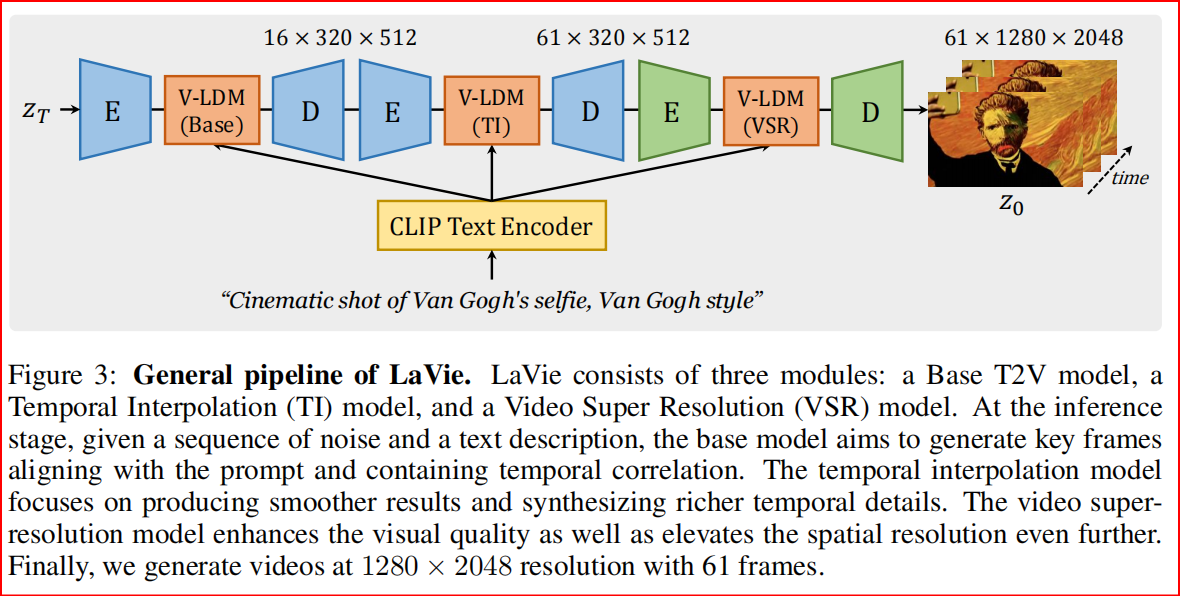
\includegraphics[width=7cm]{Image/LAVIE pipeline.png}
    \caption{LAVIE pipeline}
    \label{fig-sample}
\end{figure}
\begin{figure}[h!]
    \centering
    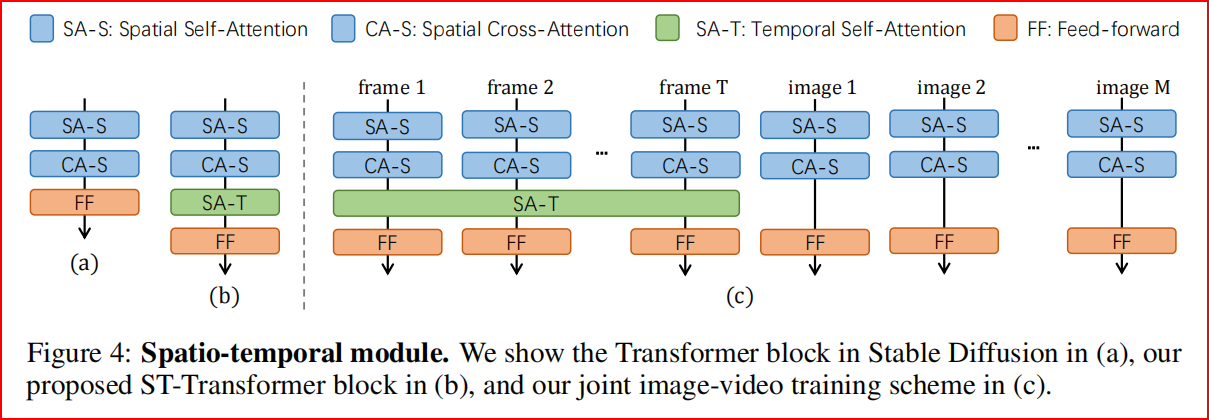
\includegraphics[width=7cm]{Image/LAVIE modification.png}
    \caption{LAVIE modification}
    \label{fig-sample}
\end{figure}

\subsubsection{SMA: Spectral Motion Alignment for Video Motion Transfer using Diffusion Models}

SMA is a novel Fourier and wavelet-transform-based motion vector refinement
and alignment framework. This includes two primary components: First, to learn
the global motion context, they propose the spectral alignment loss between predicted and ground-truth motion vectors within the wavelet domain. This facilitates the learning of multi-scale motion dynamics by leveraging rich wavelet domain representations of video considering the global frame transitions. Moreover, to mitigate the spatial artifacts and inconsistency in motion vectors, they propose 2D FFT-based motion vector refinement that aligns the amplitude and phase spectrum of ground truth and predicted motion vectors with prioritizing low-frequency components. This is because the high-frequency components in motion vectors may be associated with frame-wise non-motion-related artifacts.
\begin{figure}[h!]
    \centering
    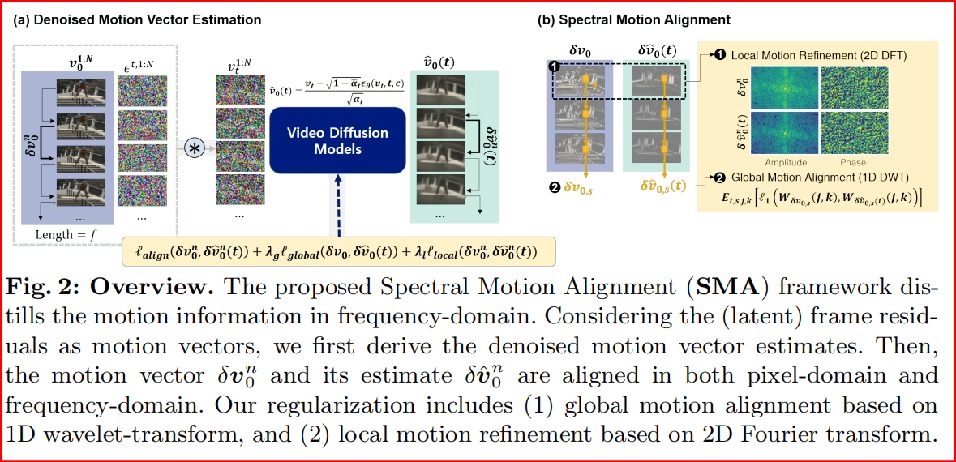
\includegraphics[width=7cm]{Image/SMA.png}
    \caption{SMA}
    \label{fig-sample}
\end{figure}

\subsubsection{LVDM:Latent Video Diffusion Models for High-Fidelity Video Generation with Arbitrary Lengths}
\begin{enumerate}
    \item[A.]General Introduction

    LVDM is a new method to generate videos, which don't need large computational resources and cause more computational expensive, while the quality and length of the videos generated by the GANs and autoregressive models were not satisfactory. It is a lightweight video diffusion model, which can synthesize high-fidelity and arbitrarily long videos from pure noise. Diffusion and denoising in a low-dimensional 3D latent space clearly outperforms previous methods in the 3D pixel space with a limited computational budget.

    First, it compress video samples to a lower-dimensional latent space by a 3D autoencoder. Then, a unified video diffusion model is designed, which can perform unconditional generation and conditional video prediction in a latent space in a network. This enables the model to self-scale the generated videos to arbitrary lengths in an autoregressive manner. In order to further improve the consistency of the generated long videos and alleviate the quality degradation caused by the cumulative error over time, this paper proposed to first sparsely generate a video using an autoregressive model, and then interpolate it to a higher frame rate by an interpolating diffusion model
\end{enumerate}
\begin{figure}[h!]
    \centering
    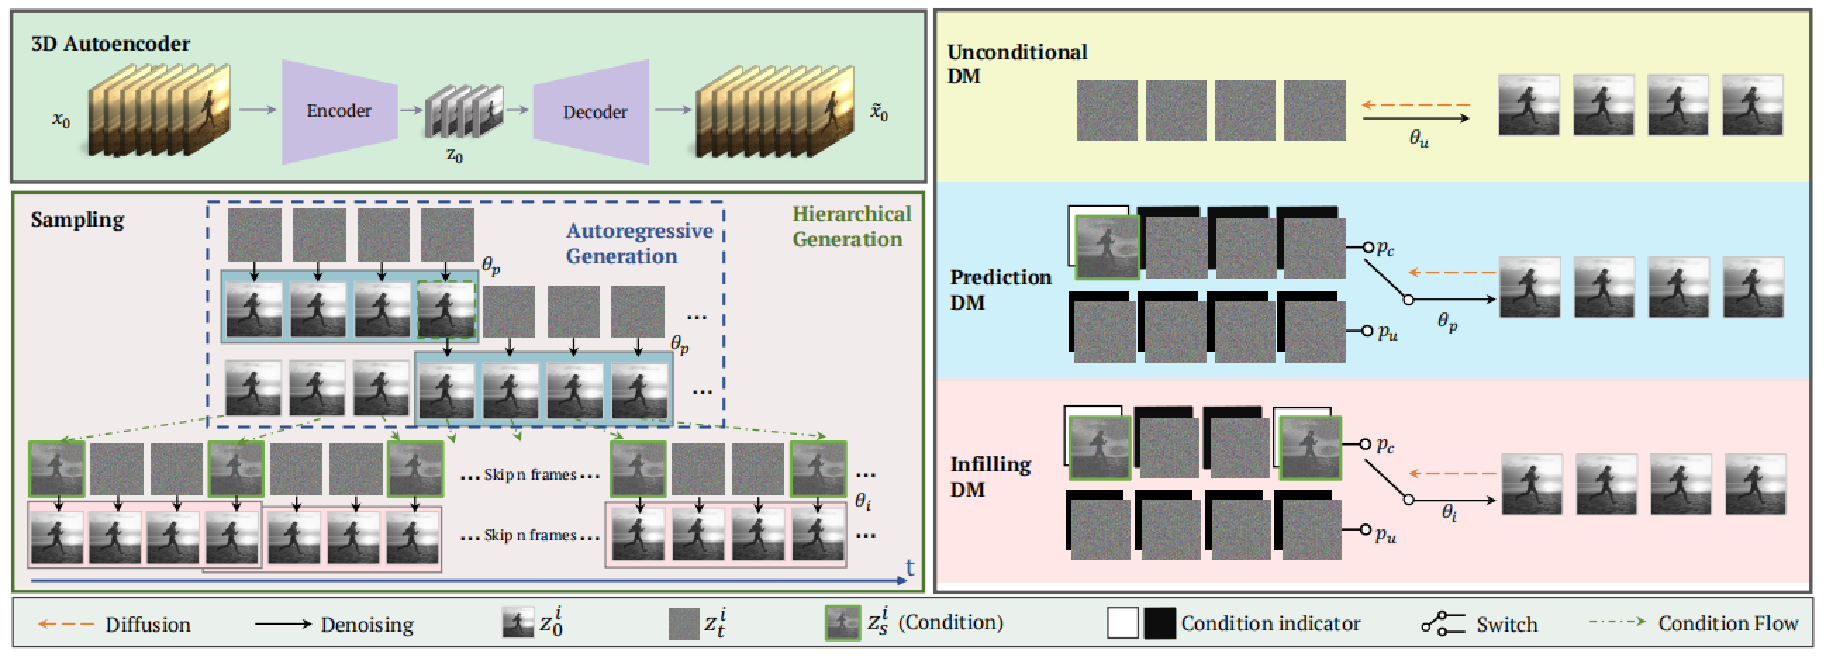
\includegraphics[width=7cm]{Image/LVDM Method.jpg}
    \caption{LVDM}
    \label{fig-sample}
\end{figure}
\begin{enumerate}
    \item[B.]Video Compression
    \begin{enumerate}
        \item[a.]Video Autoencoder
        
        A lightweight 3D autoencoder is used to compress the video, including an encoder E and a decoder D, both of which consist of several layers of 3D convolutions	
    
        The training objective includes a reconstruction loss Lrec and an adversarial loss Ladv. The reconstruction loss Lrec is comprised of a pixel-level mean-squared error (MSE) loss and a perceptual-level LPIPS loss.Learned Perceptual Image Patch Similarity (LPIPS) is a metric used to evaluate the quality of images or videos, which measures the visual similarity between different images by comparing features extracted by deep learning models
    \end{enumerate}
\end{enumerate}
\begin{enumerate}
    \item[C.]Short Video Generation
    \begin{enumerate}
        \item[a.]Video Generation Backbone
        
        
    \end{enumerate}
\end{enumerate}
\begin{enumerate}
    \item[D)]Long Video Generation
    \begin{enumerate}
        \item[a.]Autoregressive Video Generation
    
    \end{enumerate}
    \begin{enumerate}
        \item[b.]Hierarchical Video Generation
    
    \end{enumerate}
    \begin{enumerate}
        \item[c.]Conditional Latent Perturbation
    
    \end{enumerate}
\end{enumerate}



\subsection{Video Interpolation}
Throughout the last semester, we conducted experiments on MCVD and LDMVFI, and the results showed that LDMVFI outperformed MCVD in both inference speed and restoration accuracy.This semester, we did another experiment on DQBC(Video Frame Interpolation with Densely Queried Bilateral Correlation). Firstly, the Densely Queried Bilateral Correlation (DQBC) is extracted. The Motion Generation Module (MGM) generates preliminary motion fields with the help of DQBC. The Motion Refinement Module (MRM) refines and up-samples the motion fields to full size and produces a preliminary occlusion map O. For DQBC module, tokens in F1 are taken as queries and tokens in local windows on several down-sampled F0 are taken as keys to compute similarities. The unilateral correlation embeddings are then enhanced by the enhancement block and spatially aligned by the feature distributing operation. DQBC is the concatenation of two bilateral correlation embeddings.
\begin{figure}[h!]
    \centering
    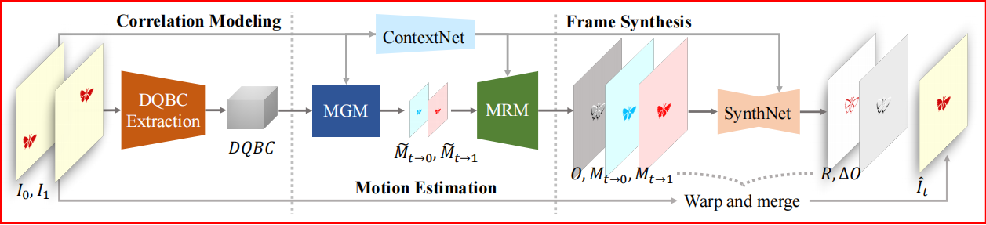
\includegraphics[width=7cm]{Image/DQBC pipeline.png}
    \caption{DQBC pipeline}
    \label{fig-sample}
\end{figure}
\begin{figure}[h!]
    \centering
    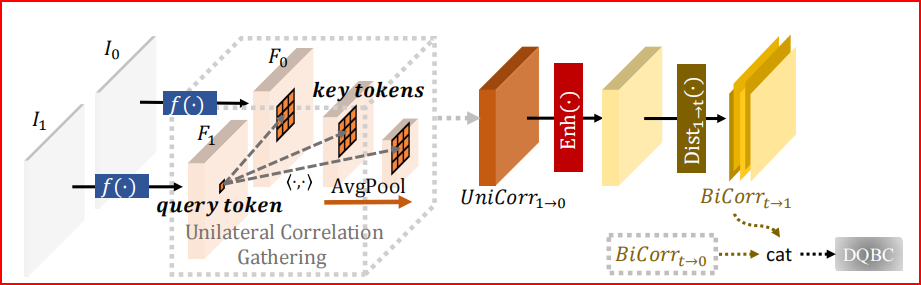
\includegraphics[width=7cm]{Image/DQBC.png}
    \caption{DQBC}
    \label{fig-sample}
\end{figure}


\section{Video Generation}

\subsection{LAVEI}
Below is the result of LAVEI with prompt of a close-up view of an eye undergoing a cataract surgery incision with a puncture knife.
\begin{figure}[h!]
    \centering
    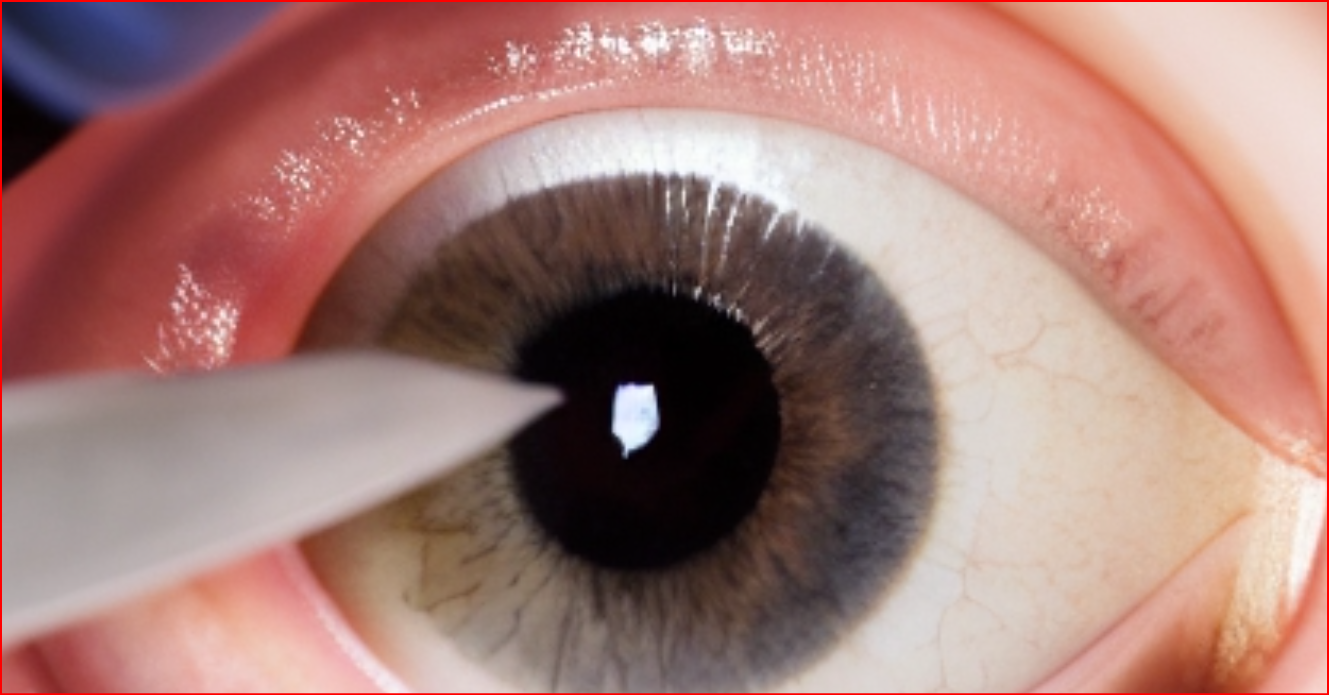
\includegraphics[width=7cm]{Image/LAVEI result.png}
    \caption{LAVEI result}
    \label{fig-sample}
\end{figure}

\section{Video interpolation}
\subsection{Review}

\subsubsection{MCVD}
The model is difficult to train, has slow inference speed, produces poor interpolation results, fails to fully decode noise, and struggles to learn motion features.
\begin{figure}[h!]
    \centering
    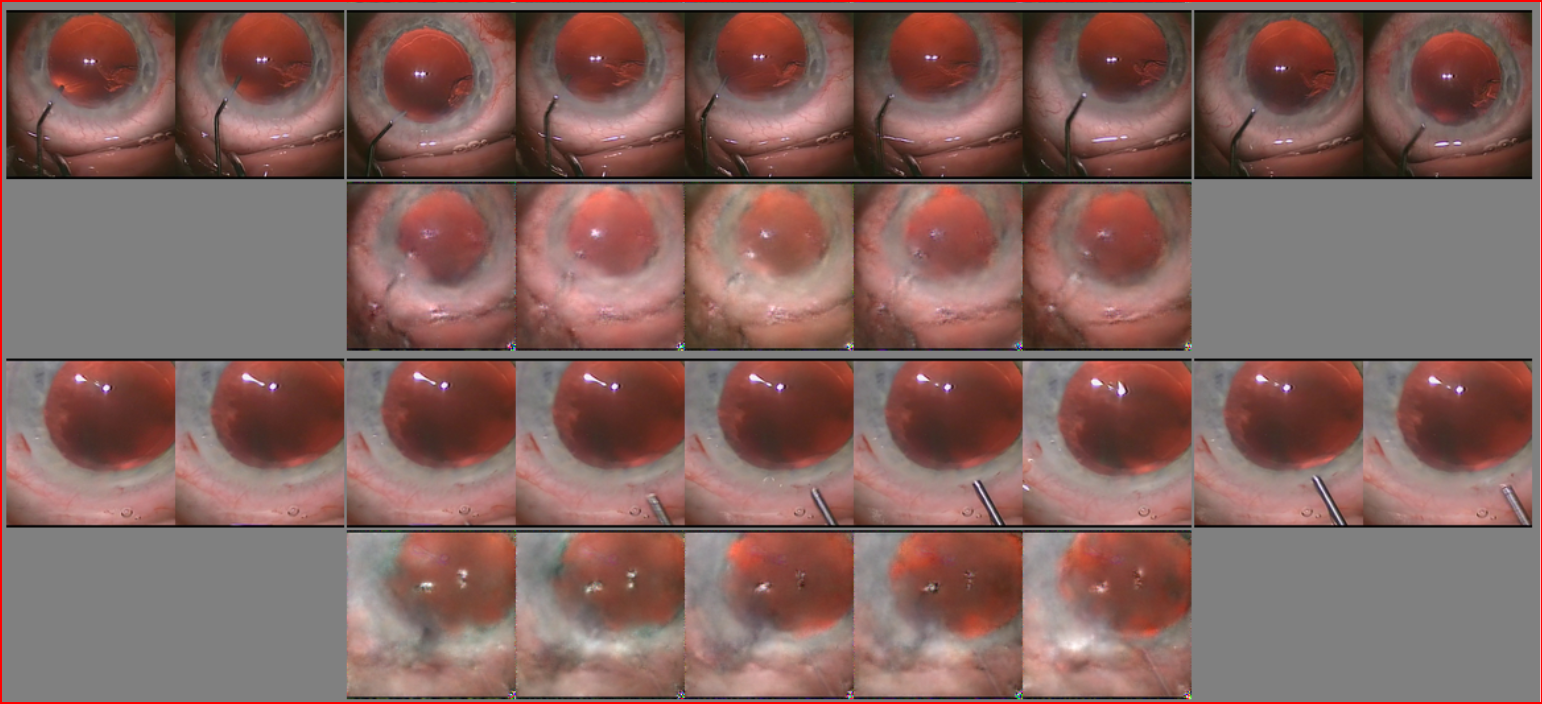
\includegraphics[width=7cm]{Image/MCVD result.png}
    \caption{MCVD result}
    \label{fig-sample}
\end{figure}

\subsubsection{LDMVFI}
The model is easier to train, has decent inference speed, achieves relatively high interpolation results, but tends to produce artifacts.
\begin{figure}[h!]
    \centering
    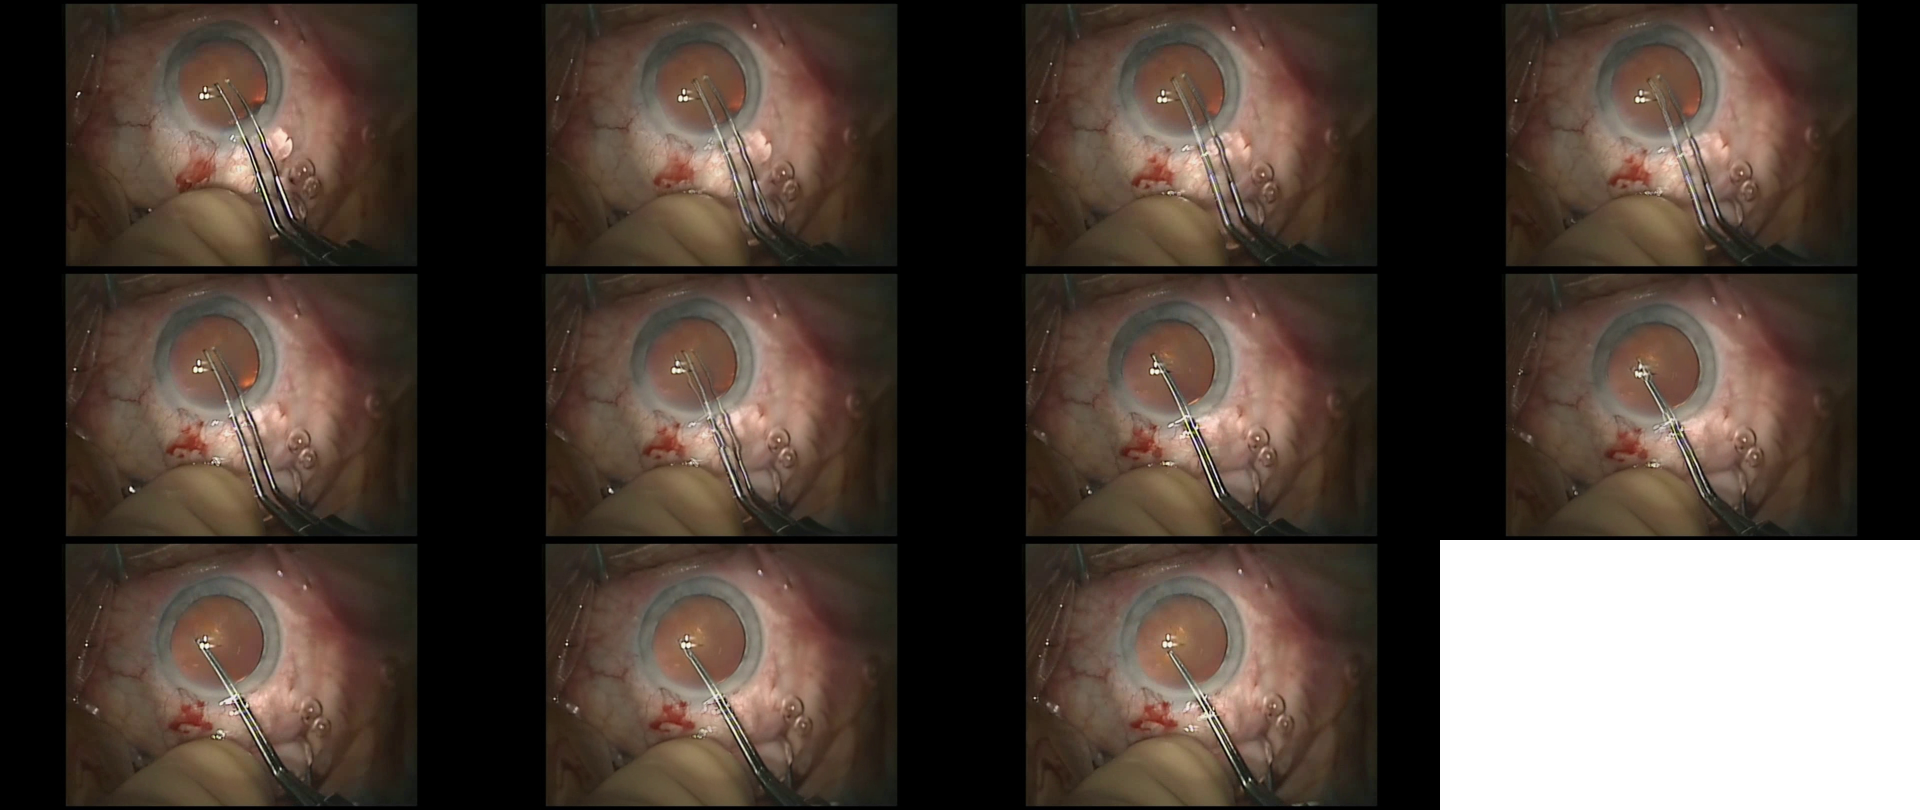
\includegraphics[width=7cm]{Image/LDMVFI result.png}
    \caption{LDMVFI result}
    \label{fig-sample}
\end{figure}

\subsection{Experiment}

\subsubsection{DQBC}
The model has fast inference speed, accurately captures the rapid motion of instruments, but the motion part is blurred.
\begin{figure}[h!]
    \centering
    \begin{subfigure}[b]{0.3\textwidth}
        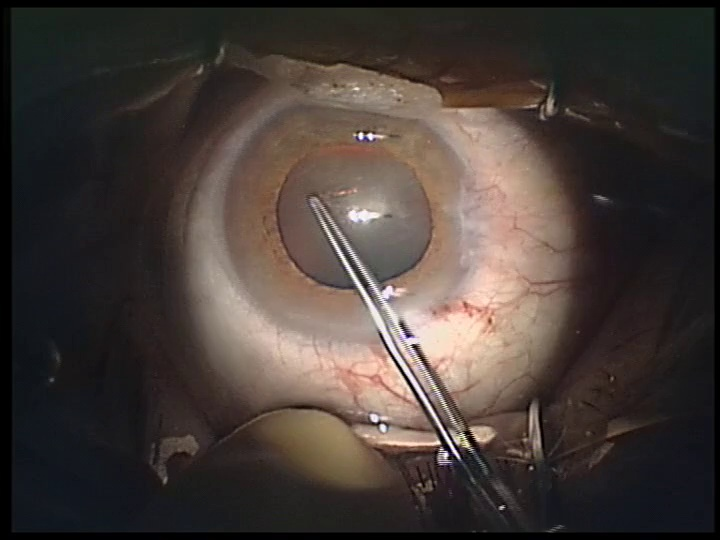
\includegraphics[width=\textwidth]{Image/DQBC result1.jpg}
        \caption{Before}
        \label{fig:dqbc1}
    \end{subfigure}
    \hfill
    \begin{subfigure}[b]{0.3\textwidth}
        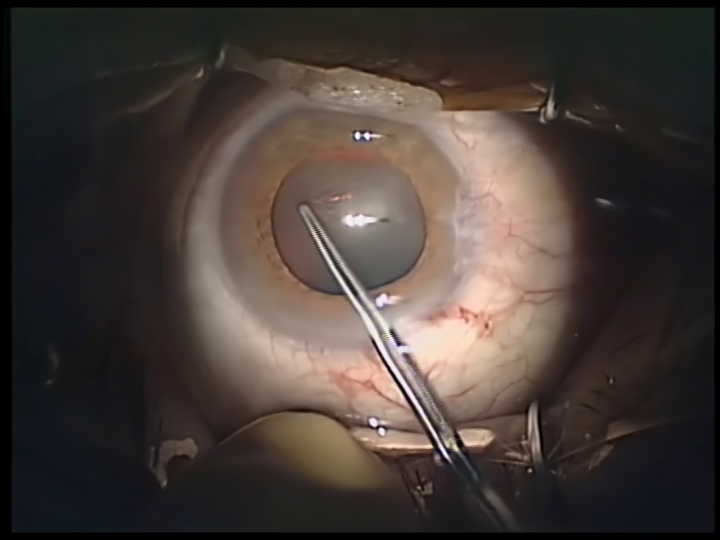
\includegraphics[width=\textwidth]{Image/DQBC result2.jpg}
        \caption{Interpolation}
        \label{fig:dqbc2}
    \end{subfigure}
    \hfill 
    \begin{subfigure}[b]{0.3\textwidth}
        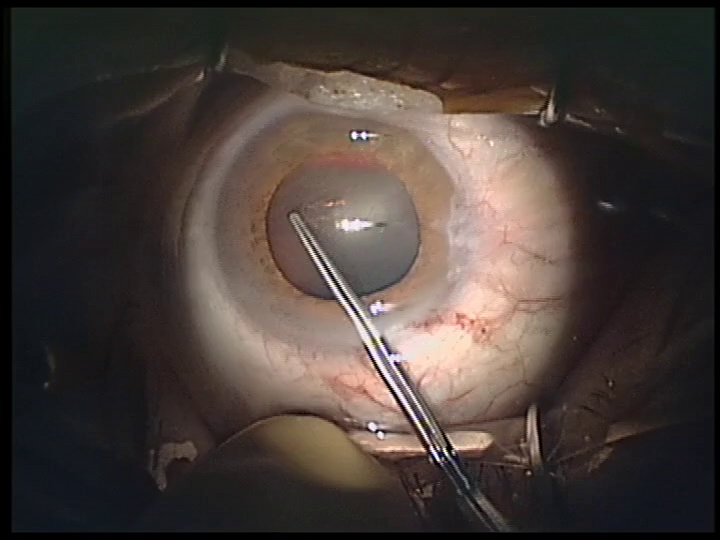
\includegraphics[width=\textwidth]{Image/DQBC result3.jpg}
        \caption{After}
        \label{fig:dqbc3}
    \end{subfigure}
    \caption{DQBC interpolation results}
    \label{fig:dqbc_results}
\end{figure}

\subsection{Comparison}
From the results, we observe that MCVD struggles with motion learning, while LDMVFI learns motion well but has some artifacts. DQBC, a non-diffusion-based model not trained on our dataset, still performs relatively well.

\section{Evaluation Criterion}

\subsection{PSNR:Peak Signal-to-Noise Ratio}
It measures the ratio between the maximum possible power of an image and the power of corrupting noise that affects its quality. A higher PSNR indicates better image quality. In PSNR*, each pixel is given equal weight in the evaluation, rather than each frame, which is crucial for assessing regions with different numbers of pixels, such as partially occluded areas.
\subsection{SSIM:Structured Similarity Index Measure}
It measures the perceptual and structural differences between two images. A higher MS value indicates a better match in terms of both visual perception and structural similarity.
\subsection{FID:Fréchet Inception Distance}
It evaluates the similarity of generated images to real ones on the feature level, with a lower FVD indicating better similarity. It is used to assess the temporal coherence of video content, in addition to the quality of each individual frame.
\subsection{CLIPSIM: CLIP Similarity}
It is utilized to output text and image similarity. In video tasks, the average similarity of each frame is taken to measure the overall performance. A higher average indicates better similarity between text and images.

\section{Further Works}
\subsection{Original pipeline}
The original pipeline is based on the Stable Diffusion model and incorporates HED (Holistically-Nested Edge Detection) to control motion. In this setup, the text-to-frame component does not learn motion directly but is guided by HED images. After generating the main frames, LDMVFI is used to interpolate the frames for a smoother and better-quality video.
\begin{figure}[h!]
    \centering
    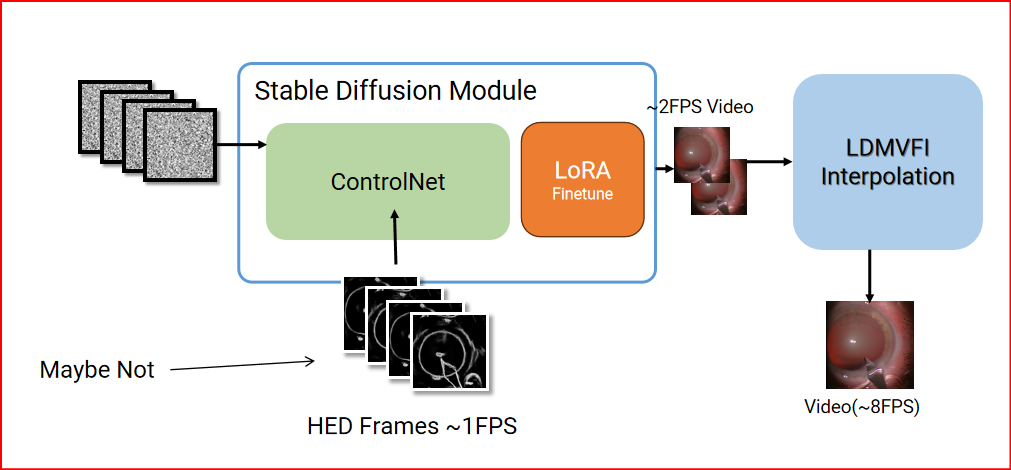
\includegraphics[width=7cm]{Image/Original pipeline.png}
    \caption{Original pipeline}
    \label{fig-sample}
\end{figure}

\subsection{Modification}
In the next six weeks, to enhance frame generation, one approach is to remove the HED control and train the Stable Diffusion model to directly learn motion. Alternatively, integrating other models that excel in motion capture could also improve the overall performance. For interpolation, to eliminate issues such as artifacts, we will incorporate the motion supervision part from DQBC into LDMVFI.

\end{document}